\section{Experiments}

\subsection{Machine Specification}
We executed the following tests using this environment:

%TODO Please Bera write down your machine spec.

\begin{itemize}
    \item \textbf{Machine}:
    \begin{itemize}
        \item Type:
        \item CPU: 
        \item RAM: 
    \end{itemize}
    \item \textbf{Software}:
    \begin{itemize}
        \item OS: 
        \item Kubernetes: 
    \end{itemize}
\end{itemize}

\subsection{Experiments Description}
The experiments have the goal of emulating different types of traffic, with the objective of showing the system behavior. The possible experiments can be performed choosing different rates following a state machine. In other words, if the user selects 4 different rates for the distribution selected the load is composed of 4 circularly executed states with the rated specified. The duration of each state is editable from the code.

So, for example, choosing a uniform distribution with all rates value such that min=max (to model the deterministic arrival process) and selecting a test with a duration of 9 minutes and rates = ([1,1];[2,2];[3,3];[5,5]) we are modelling an arrival process that generates a load with 1 message/s for 1 minute, than 2 messages/s for 1 minute, than 3 messages/s for 1 minute, than 5 messages/s for 1 minute. At this point 4 minutes has been passed so the arrival process restarts circularly from 1 message/s and so on until the end of the test.

\subsection{Experiments guide}
In this section we include a miniguide to reproduce our experiments. First of all it is necessary to clone the GitHub repository at \href{https://github.com/Berags/oris-predictive-autoscaler}{this link} (https://github.com/Berags/oris-predictive-autoscaler). To start the project is necessary, as a minimum dependancy, to have installed \href{https://minikube.sigs.k8s.io/docs/}{Minikube}. After having installed successfully Minikube, execute the following command:

\begin{table}[!htb]
\centering
\begin{tabular}{c}
\begin{lstlisting}
minikube start
\end{lstlisting}
\end{tabular}
\end{table}

then, it is sufficient to position the terminal on the directory of the project where it is present the .sh file named ./start.sh and execute:

\begin{table}[!htb]
\centering
\begin{tabular}{c}
\begin{lstlisting}
./start.sh
\end{lstlisting}
\end{tabular}
\end{table}
the file start.sh contains all the instruction necessary to build and run our project (i.e. all the containers and components). Don't mind if it takes a while, it is perfectly normal due to the project complexity. At this point, as reported in \guillemotleft port-forward.sh\guillemotright \ you can monitor:
\begin{itemize}
  \item The RabbitMQ queue at \guillemotleft http://localhost:15672\guillemotright
  \item Prometheus at \guillemotleft http://localhost:9090\guillemotright
  \item Grafana (with all the dashboards of interest shown below) at \guillemotleft http://localhost:3000\guillemotright, the default username and password is \verb|admin|.
  \item Kafdrop (for the Kafka queue) at \guillemotleft http://localhost:9000\guillemotright
\end{itemize}

At this point everything is ready to start the tests. In order to do it, go ( we suggest with an additional terminal window) in the folder of \guillemotleft build-and-run.sh\guillemotright \ that is inside the \guillemotleft k6 \guillemotright folder and execute the file with
\begin{table}[!htb]
\centering
\begin{tabular}{c}
\begin{lstlisting}
./build-and-run.sh
\end{lstlisting}
\end{tabular}
\end{table}

\begin{lstlisting}[mathescape]
1. Exponential
2. Poisson ($\lambda$<100)
3. Uniform (Use min = max for deterministic)
4. Erlang (k, $\lambda$)
5. Exit
----------------------------
Insert your choice:
\end{lstlisting}

In this way in the console is shown the test menu from which you can choose the distribution of the load you want to simulate. The available distributions are the above. Then, remains only to choose the rates as described before and how you can see below. Then, the test starts and the console reports some logs. To monitor the entire system consult the addresses above. 

\subsubsection{Experiment personalization}

Copying the repository you can essentially modify the code as you prefer but if you want to modify the transition time is sufficient to modify the following instruction:

\begin{table}[!htb]
\centering
\begin{tabular}{c}
\begin{lstlisting}
const transitionTime = DistributionFactory.getDeterministic(60);
\end{lstlisting}
\end{tabular}
\end{table}

in rabbitmq-test.js and with \guillemotleft 60\guillemotright \ that are the seconds of permanence in each state. If you are not interested in a deterministic transition you can substitute it, for example, with an Exponential one with:

\begin{table}[!htb]
\centering
\begin{tabular}{c}
\begin{lstlisting}
const transitionTime = DistributionFactory.getExponential(20);
\end{lstlisting}
\end{tabular}
\end{table}


Please notice ho we modeled arrival processes of our interest using the js library included in the code repo under k6/lib (all the documentation inside), but eventually you can use also the others distributions supported.

\subsubsection{Setup Details}

If you are wondering what are the uses of others \textit{.sh} files, this is the right section. Essentially, the fundamental ones are \guillemotleft start.sh\guillemotright \ and \guillemotleft build-and-run.sh\guillemotright \ but since ./start.sh does a lot of work and when something goes wrong is not everytime necessary to rebuild everything, we provided \guillemotleft port-forward.sh\guillemotright \ for the port forwarding only and \guillemotleft delete\_and\_deploy\_sirio.sh\guillemotright \ to, as its name suggests, delete and redeploy only sirio.

\subsection{Model of Arrivals}
For all the test, we modeled in Sirio the Arrival process as an Exponential with parameter $\lambda$ equal to the inverse of the average inter-arrival time of the messages in the queue (or $\lambda$ equals to the average messages per second, it's the same). 

We also tried using Bernstein phase types, but we encountered a problem that stopped it. It seems that the Sirio model of a Bernstein phase type uses a rapidly increasing amount of RAM while increases the number of phases. For instance, we tried 50 phases and the scaler tried to instance in the heap more than 768MB, making the pods overflow and be killed by Kubernetes. With a lower number of phases, we didn't achieve a good enough approximation to be used in the scaler. In the other hand, trying to extend the amount of RAM available to the Sirio pod make the machine's OS trashing most of the time.

In addition to that, we found the approximation with the exponential more that capable to a uniform arrival rate. Then, having a microservice controller that consumes so much resource seem odd and counterproductive.

\subsection{Rejection Rate Calculation}
Here we want to discuss how we calculated the rejection rate, and the reasons to choose it. For our experiments, we wanted to calculate a relative rejection rate. In fact, we consider this approach more robust if compared to an absolute rejection rate target.

The rejection rate, at least in terms of expected value, can be defined as: \textit{the probability that a packed get rejected by the queue}. To verify this condition, two pre-conditions must be true:
\begin{itemize}
    \item The Queue is full.
    \item The arrival process is habilitated to push a new message.
    \item The arrival process extracts a time to fire smaller than the service process.
\end{itemize}

Considering a stochastic model expressed in term of a Stochastic Time Petri Net (STPN), we are interested in only three elements: the place of the queue, the last transition of the arrival process that goes into the queue, and the first transition of the service that pulls from the queue (most of the time the service is represented with only a transition). For this problem we assume that the stochastic properties of the model depends only on the marking state. So, let $R$ be the event of a rejection, $Q=q_{max}$ the event of a marking with the queue full, $A$ the event of a marking where the last arrival transition has a token as a precondition, $t_a$ and $t_s$ the values sampled from the arrival and service transitions, and $\lambda_a$ and $\lambda_s$ the arrival and service rate respectively, from the previous conditions we can derive the equation \ref{eq:rejection}:

\begin{equation}
    \label{eq:rejection}
    \begin{split}        
    P(R)& =P(Q=q_{max} \land A\land t_a<t_s)\\
    & = P(t_a<t_s|Q=q_{max})P(Q=q_{max} \land A)
    \end{split}
\end{equation}

Considering that we used a Markovian model, the arrival and service transitions samples their times to fire form exponential transitions. So, let $\lambda_a$ and $\lambda_s$ of two transition when the queue is full, we can rewrite equation \ref{eq:rejection} as \ref{eq:rejection_exp}:
\begin{equation}
    \label{eq:rejection_exp}
    \begin{split}
    P(R) & =  P(t_a<t_s|Q=q_{max}\land A)P(Q=q_{max}\land A) \\
     & = P(Exp(\lambda_a)<Exp(\lambda_s))P(Q=q_{max}\land A)
    \end{split}
\end{equation}

Can be easily derived the probability of an exponential samples before another as in equation \ref{eq:first_exp}, the final rejection rate formula it \ref{eq:rejection_fin}.
\begin{gather}
P(Exp(\lambda_a)<Exp(\lambda_s)) = \frac{\lambda_a}{\lambda_a + \lambda_s} \label{eq:first_exp}\\
P(R)=\frac{\lambda_a}{\lambda_a + \lambda_s}P(Q=q_{max}\land A) \label{eq:rejection_fin}
\end{gather}

Considering that given a closed model Sirio is capable to enumerate all the reachable states, using the steady state analysis we can get the probability of having a state where the queue is full and the arrival transition is enable, while using the \textit{MarkingExpresions} getting transition rates is trivial.

Here below, to highlight how this formula can be translated in practice, is reported the code that calculated the rejection rate.
\begin{lstlisting}
BigDecimal rejection = BigDecimal.ZERO;
Map<Marking, BigDecimal> results = RegSteadyState.builder().build().compute(pn, m).getSteadyState();
for (Marking tmp : results.keySet()) {
    if (tmp.getTokens(queuePlace) == queue.getSize() && pn.isEnabled(arrivalTransition, tmp)) {
        BigDecimal currentRejection = results.get(tmp);

        BigDecimal arrivalRate = extractLambda(arrivalTransition, tmp).setScale(8, RoundingMode.HALF_UP);
        BigDecimal serviceRate = extractLambda(serviceTransition, tmp).setScale(8, RoundingMode.HALF_UP);

        currentRejection = currentRejection.multiply(arrivalRate).divide(arrivalRate.add(serviceRate), 8, RoundingMode.HALF_DOWN);

        rejection = rejection.add(currentRejection);
    }
}
return rejection;
\end{lstlisting}

\subsection{Experiments Setup}
In all tests we set some common parameters:
\begin{enumerate}
    \item Rejection Rate: 5\%.
    \item Service Rate: 1.
    \item Duration of states in the arrival process: 60s.
    \item Total test duration: \textbf{TODO Bera insert the exact experiment time}.
\end{enumerate}

For the experiments with constant arrival time, we defined a state machine with the following parameters: [0.33,0.33],[0.2,0.2],[0.11,0.11],[1,1],[0.14,0.14]. In this, for every state we sample the same inter arrival time with the following expected messages per second: 3, 5, 9, 1 and 7. Considering that the state machine is cyclic, this behavior repeats periodically.

On the other hand, we tried a stochastic workload using exponential as inter arrival time distributions in the machine states. The parameters used are: 3, 5, 7, 1, 9. These are also the expected messages per second of the respectively state.

In this report, we separated the logic of establishing the optimal number of replicas (the Recommender) from the one that communicates with Kubernetes (Updater). This allows to apply different scaling logics to the workers. In the following we will confront an immediate application of the recommendation, versus a sliding window approach that waits a series of downscale recommendation before applying it.

\subsection{Results}
\subsubsection{Immediate Apply of Recommendations}

In executing this experiment, both for constant and exponential arrival rates, we measure the arrived and rejecte messages in figure \ref{}.
This behavior is correctly shown in image \ref{fig:uniform_messages}.
\begin{figure}[H]
	\begin{subfigure}{0.85\linewidth}
	    \centering
	    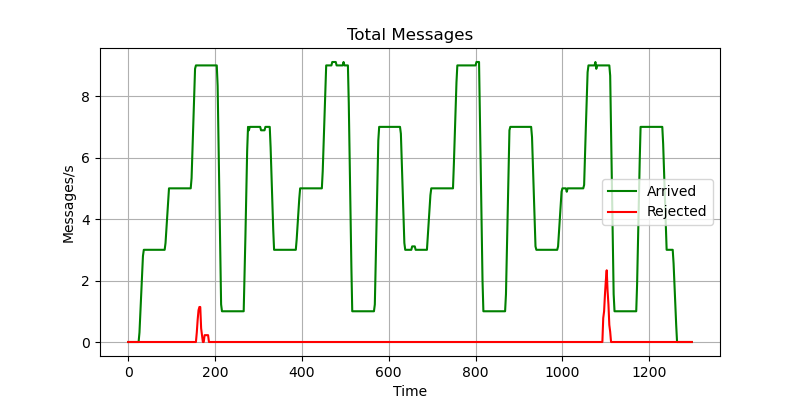
\includegraphics[width=0.85\linewidth]{images/default/constant/messages.png}
	    \caption{Arrived and Rejected messages per second to the Queue.}
	    \label{fig:uniform_messages}
	\end{subfigure}
	\begin{subfigure}{0.85\linewidth}
	    \centering
    		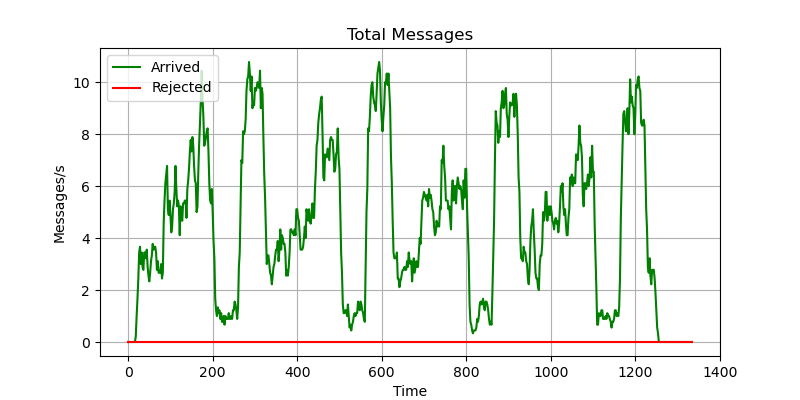
\includegraphics[width=0.85\linewidth]{images/default/exponential/messages.png}
	    \caption{Arrived and Rejected messages per second to the Queue.}
    		\label{fig:uniform_messages}
	\end{subfigure}
\end{figure}
As said, the goal of the control is to keep a rejection rate below 5\%. In figure \ref{fig:uniform_rejection} is reported the cumulative rejection rate through time. To obtain this graph, we calculated the cumulative quantity of rejected messages, and then divided for the corresponding cumulative value of arrived messages. The exact final rejection rate is \textbf{2.8\%}.

\begin{figure}[H]
    \centering
    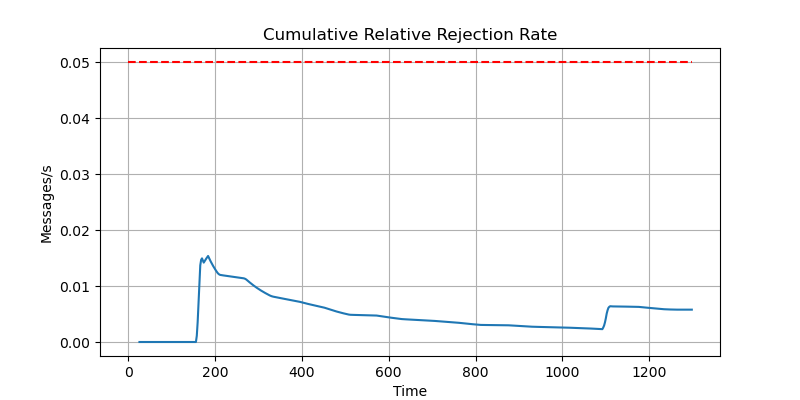
\includegraphics[width=0.85\linewidth]{images/default/constant/rejection_cumulative.png}
    \caption{Cumulative rejection rate.}
    \label{fig:uniform_rejection}
\end{figure}

We can see the rise in rejections after increasing the amount of arriving messages, but after that a descent below the specified target.

Another measure that we consider relevant is the cost inefficiency of the scaler implementation. Due to the fact that creating and destructing pods isn't an immediate operation, Kubernetes takes some time to set the number of replicas to the number prescribed by the Sirio Scaler. This lag in control can be appreciated in figure \ref{fig:uniform_pods}.
\begin{figure}[H]
    \centering
    \begin{subfigure}{0.85\textwidth}
        \centering
        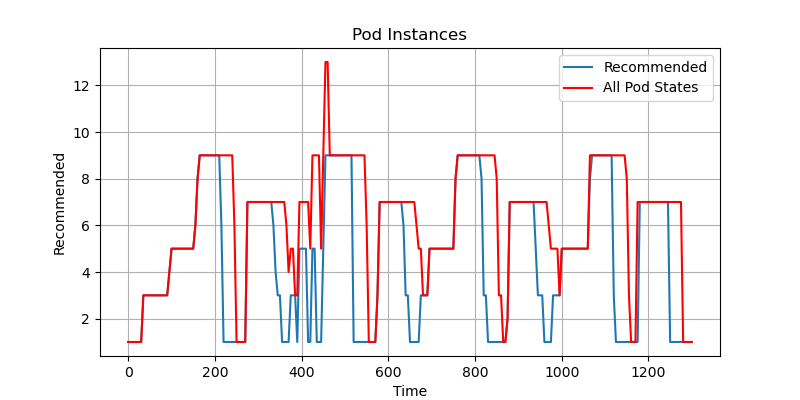
\includegraphics[width=\textwidth]{images/default/constant/pods.png}
        \caption{In blue the number of pods prescribed by the scaler, the red one pods in all states.}
        \label{fig:uniform_pods}
    \end{subfigure}
    \begin{subfigure}{0.85\textwidth}
        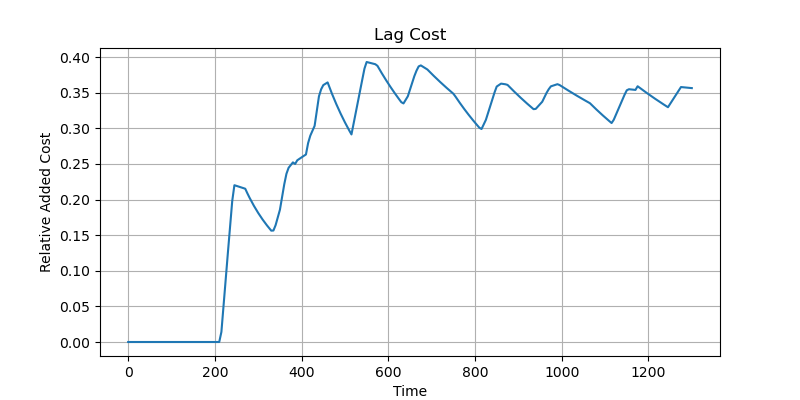
\includegraphics[width=\linewidth]{images/default/constant/lag_cost_cumulative.png}
        \caption{At every time $t$, we calculate the inefficiency from starting time.}
        \label{fig:uniform_inefficiency}
    \end{subfigure}
\end{figure}

In figure \ref{fig:uniform_inefficiency} is reported the inefficiency while the system goes; in the followings more details in how this curve is calculated. To understand this calculation, we need to start from how cost is defined. We choose to measure cost without loss of generality in the unit of $pods \cdot time$, so that the cost of the system is both proportional to the quantity of resources used and the time we used. It's worth noting that this type of billing is common in many types of cloud providers. For example, a system that executes 5 pods for 3 seconds has a cost of 15. So, given any sequence of measured pods $pods_i$ for $i=1,\dots,t$, with a sampling period of $T_s$, the total cost of the system is calculated as \ref{eq:cost}:
\begin{equation}
    \label{eq:cost}
    C = T_s\sum_{i=1}^{t}pods_i
\end{equation}

So, be $C_{preb}$ the prescribed cost obtained by the sequence of pods dictated by the Sirio Scaler, and $C_{real}$ the real cost of all existing pods, we calculated the relative inefficiency as in equation \ref{eq:inefficiency}:
\begin{equation}
    \label{eq:inefficiency}
    I =\frac{C_{real} - C_{preb}}{C_{preb}} = \frac{C_{real}}{C_{preb}} - 1
\end{equation}

Giving the formulas in \ref{eq:cost} and \ref{eq:inefficiency}, both can be calculated for a particular time $t_0$ by truncating the sequence $pods_i$ for $i\leq t_0$.

Note that for how we defined $I$, it can be smaller than 1 in theory. In practice, we consider initializing pods for the actual cost, and making that it's very unlikely that Kubernetes waits so much to start creating them, this eventuality is negligible. However, in equation \ref{eq:inefficiency} we can force the numerator to be bigger or at least equal to the denominator.

We want to state that this measure of inefficiency not necessary means a bad implementation, but only a measure of the difference between a perfect control and the actual one. In fact, this isn't calculated in reference to a commonly used control or any other type.

\subsubsection{Sliding Window}
We also decided to test the system with a state machine composed by exponential distributions. In this case, the states of the machine are associated with these parameters: 2,5 and 10 (The expected value of messages per second in this state are the same). 

The result in terms of arrived and rejected messages is reported in figure \ref{fig:exponential_fast_messages}, and with it the rejection rate in figure \ref{fig:exponential_fast_rejection}:

\begin{figure}[H]
    \centering
    \begin{subfigure}{0.85\linewidth}
        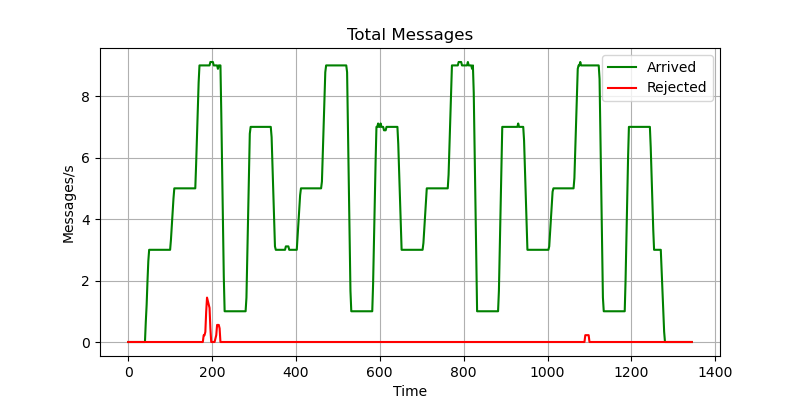
\includegraphics[width=\linewidth]{images/sliding_window/constant/messages.png}
        \caption{Arrived and Rejected messages per second to the Queue.}
        \label{fig:exponential_fast_messages}
    \end{subfigure}
    \begin{subfigure}{0.85\linewidth}
        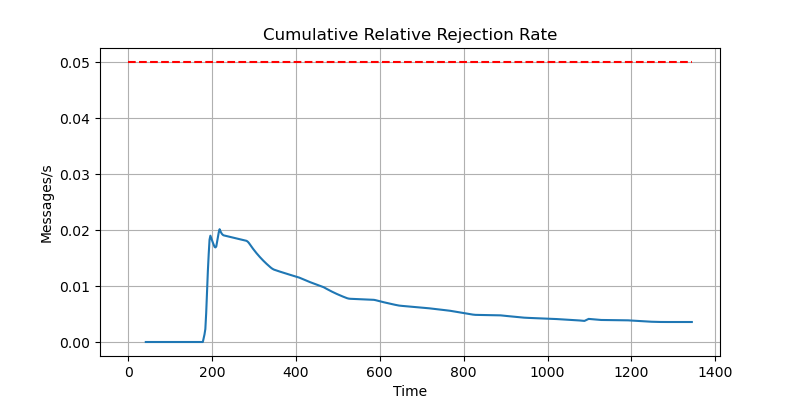
\includegraphics[width=\linewidth]{images/sliding_window/constant/rejection_cumulative.png}
        \caption{Cumulative rejection rate.}
        \label{fig:exponential_fast_rejection}
    \end{subfigure}
\end{figure}
In this case, the surge in rejection came later. This explains why the peak is much lower. In the end, the final rejection rate is \textbf{1.86\%}.

As we can see in figure \ref{fig:exponential_fast_inefficiency}, that the inefficiency in the case of the exponential is greater, even if confronted with the \textit{equivalent} (in terms of expected values of messages per second in the states) uniform case. 

\begin{figure}
    \centering
    \begin{subfigure}{0.85\textwidth}
        \centering
        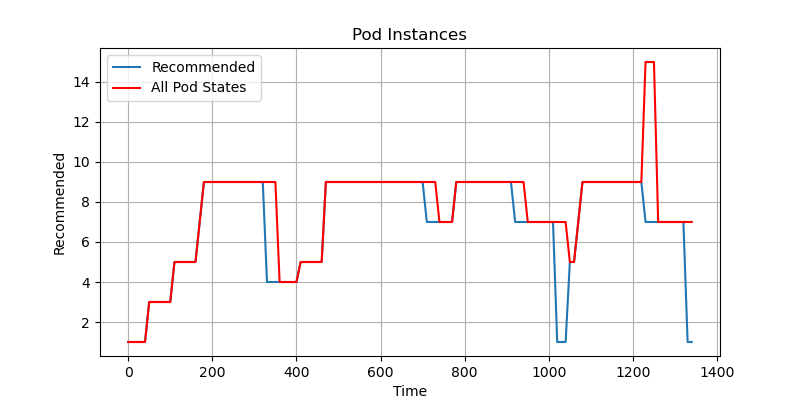
\includegraphics[width=\textwidth]{images/sliding_window/constant/pods.png}
        \caption{In blue the number of pods prescribed by the scaler, the red one pods in all states.}
        \label{fig:exponential_fast_pods}
    \end{subfigure}
    \begin{subfigure}{0.85\textwidth}
        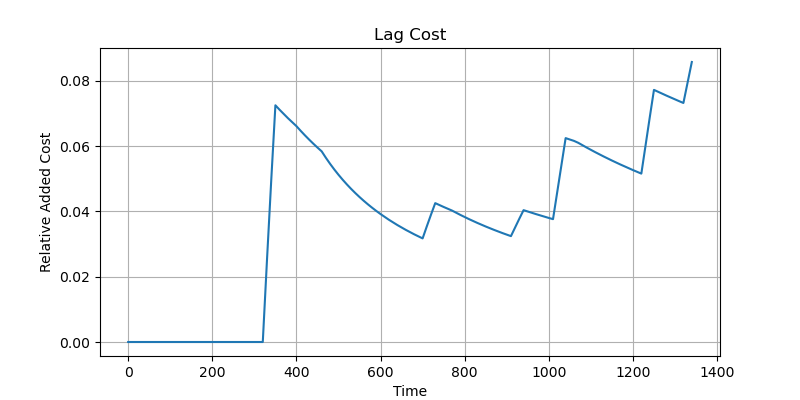
\includegraphics[width=\linewidth]{images/sliding_window/constant/lag_cost_cumulative.png}
        \caption{At every time $t$, we calculate the inefficiency from starting time.}
        \label{fig:exponential_fast_inefficiency}
    \end{subfigure}
\end{figure}

A possible reason for a greater inefficiency can be found in the variance of the stochastic process. In fact, a uniform with the maximum and minimum parameter equal (so a deterministic inter-arrival) has zero variance. In this scenario, Sirio Scaler should not change the prescribed replicas. In the other hand, having an instantaneous (or an average in a short time period) messages arrived per second can make the Sirio Scaler change a little the prescription. So, due to creation or terminating time we have slightly more pods than required.
